\documentclass[12pt]{report}
\usepackage[margin=1in]{geometry}
\usepackage[compact,raggedright]{titlesec}
\usepackage{setspace} % for single/doublespacing commands
\usepackage{graphicx} % including graphics
% \usepackage{sectsty} % sexy section headings
\usepackage{pdfpages} % including multipage pdfs
\usepackage[export]{adjustbox} % for graphic frames and center
\usepackage{siunitx}
\usepackage[numbered]{matlab-prettifier} % including matlab w/ syntax highlighting
\usepackage[T1]{fontenc} % prettier matlab font
\usepackage{xfrac} % more legible inline fractions (\sfrac)
\usepackage{lmodern} % font package for above
\usepackage{multicol} % multiple columns
\usepackage[justification=centering]{caption} % figure captions (force centering)
\usepackage{amsmath} % more math symbols and shit
\usepackage{enumitem} % add arguments for enumerate to change style
\usepackage{subcaption} % subfigures with list of figure support
% \usepackage{subfigure}
\usepackage{multirow}
\usepackage{mathtools}
\usepackage{booktabs}
\usepackage{color}
\usepackage{ulem}
\usepackage{blindtext}
\usepackage[numbers]{natbib}
\usepackage{contour}
\usepackage{tabularx}
\usepackage{circuitikz} % drawing fancy shit
\usepackage{cancel} % arrow and cross math cancel symbol
\usepackage{lineno}
\usepackage{framed}
\usepackage{amssymb} % special math symbols
\usepackage{listings}
\usepackage{array}
\usepackage{BOONDOX-cal} % fancy mathtype script
\usepackage{fancyhdr}
\usepackage{flowchart}
\usepackage{color, colortbl}
\usepackage{tocloft}
\usepackage{url}
\usepackage{etoolbox}
\usepackage[usestackEOL]{stackengine}
\usepackage{caption}
% \usepackage{hyperref}

\setlength{\parskip}{\baselineskip}%
\setlength{\parindent}{0pt}%

\setcounter{secnumdepth}{5}
\renewcommand{\bibname}{References}
\sisetup{output-exponent-marker=\ensuremath{\mathrm{e}}}
\newcommand{\PreserveBackslash}[1]{\let\temp=\\#1\let\\=\temp}
\newcolumntype{C}[1]{>{\PreserveBackslash\centering}p{#1}}
\newcolumntype{R}[1]{>{\PreserveBackslash\raggedleft}p{#1}}
\newcolumntype{L}[1]{>{\PreserveBackslash\raggedright}p{#1}}
\lstMakeShortInline[style=Matlab-editor]| % matlab inline escape character
\graphicspath{{images/}}
\renewcommand\thesection{\arabic{section}}
\renewcommand\labelitemi{---}
\lstset{numberstyle=\ttfamily\small\color{gray}}
\renewcommand\linenumberfont{\ttfamily\small\color{gray}}
\setlength\linenumbersep{6mm}
\hbadness=99999  % or any number >=10000
\apptocmd{\sloppy}{\hbadness 10000\relax}{}{}
\usetikzlibrary{arrows,calc,patterns,angles,quotes}
% \usetikzlibrary{shapes.geometric}
% \usetikzlibrary{decorations.pathmorphing,decorations.pathreplacing} % for snakes!
% \usetikzlibrary{positioning, circuits.logic.US}
\newcommand{\Lag}{\mathcal{L}} % lagrangian L

\apptocmd{\sloppy}{\hbadness 10000\relax}{}{}
\setlength{\cftbeforetoctitleskip}{-2em}
\setlength{\cftbeforeloftitleskip}{-2em}
\setlength{\cftbeforelottitleskip}{-2em}
% \allsectionsfont{\raggedright} % w/ secsty
\setlist[enumerate]{wide=0pt, widest=99,
                    leftmargin=\parindent,topsep=0pt,partopsep=0pt,
                    label=\thesubsubsection.\alph*,font=\itshape}

\newcommand{\hiddensubsection}[1]{
  \stepcounter{subsection}
  \subsection*{\arabic{section}.\arabic{subsection}\hspace{1em}{#1}}
}
\newcommand{\hiddenappsec}[1]{
  \stepcounter{section}
  \subsection*{\Alph{section}\hspace{1em}{#1}}
}
\newcommand{\hiddenappsub}[1]{
  \stepcounter{subsection}
  \subsection*{\Alph{section}.\Roman{subsection}\hspace{1em}{#1}}
}

\titlespacing\section{0pt}{0pt}{-5pt}
\titlespacing\subsection{0pt}{0pt}{-5pt}
\titlespacing\subsubsection{0pt}{0pt}{-5pt}

\AtBeginEnvironment{thebibliography}{\def\UrlFont{\normalfont\itshape}}

\DeclareCaptionFormat{cont}{#1 (cont.)#2#3\par}

\DeclareCaptionLabelFormat{r-parens}{Figure \thefigure#2:} %Define our custom label

% \captionsetup{font=footnotesize} % The general caption settings
\captionsetup[sub]{              % The subcaption settings
    labelformat=r-parens}        % Use our custom label format

% \renewcommand{\thesubfigure}{\thefigure\alph{subfigure}}
% \looseness=-1 % for one-liners bleeding off into the next page

\begin{document}
\normalem
\begin{titlepage}
\flushleft
\doublespacing
\Large
\textsc{Test Document} \\
\normalsize
Trey Dufrene, Zack Johnson, David Orcutt, Alan Wallingford, Ryan Warner
\vfill
\center
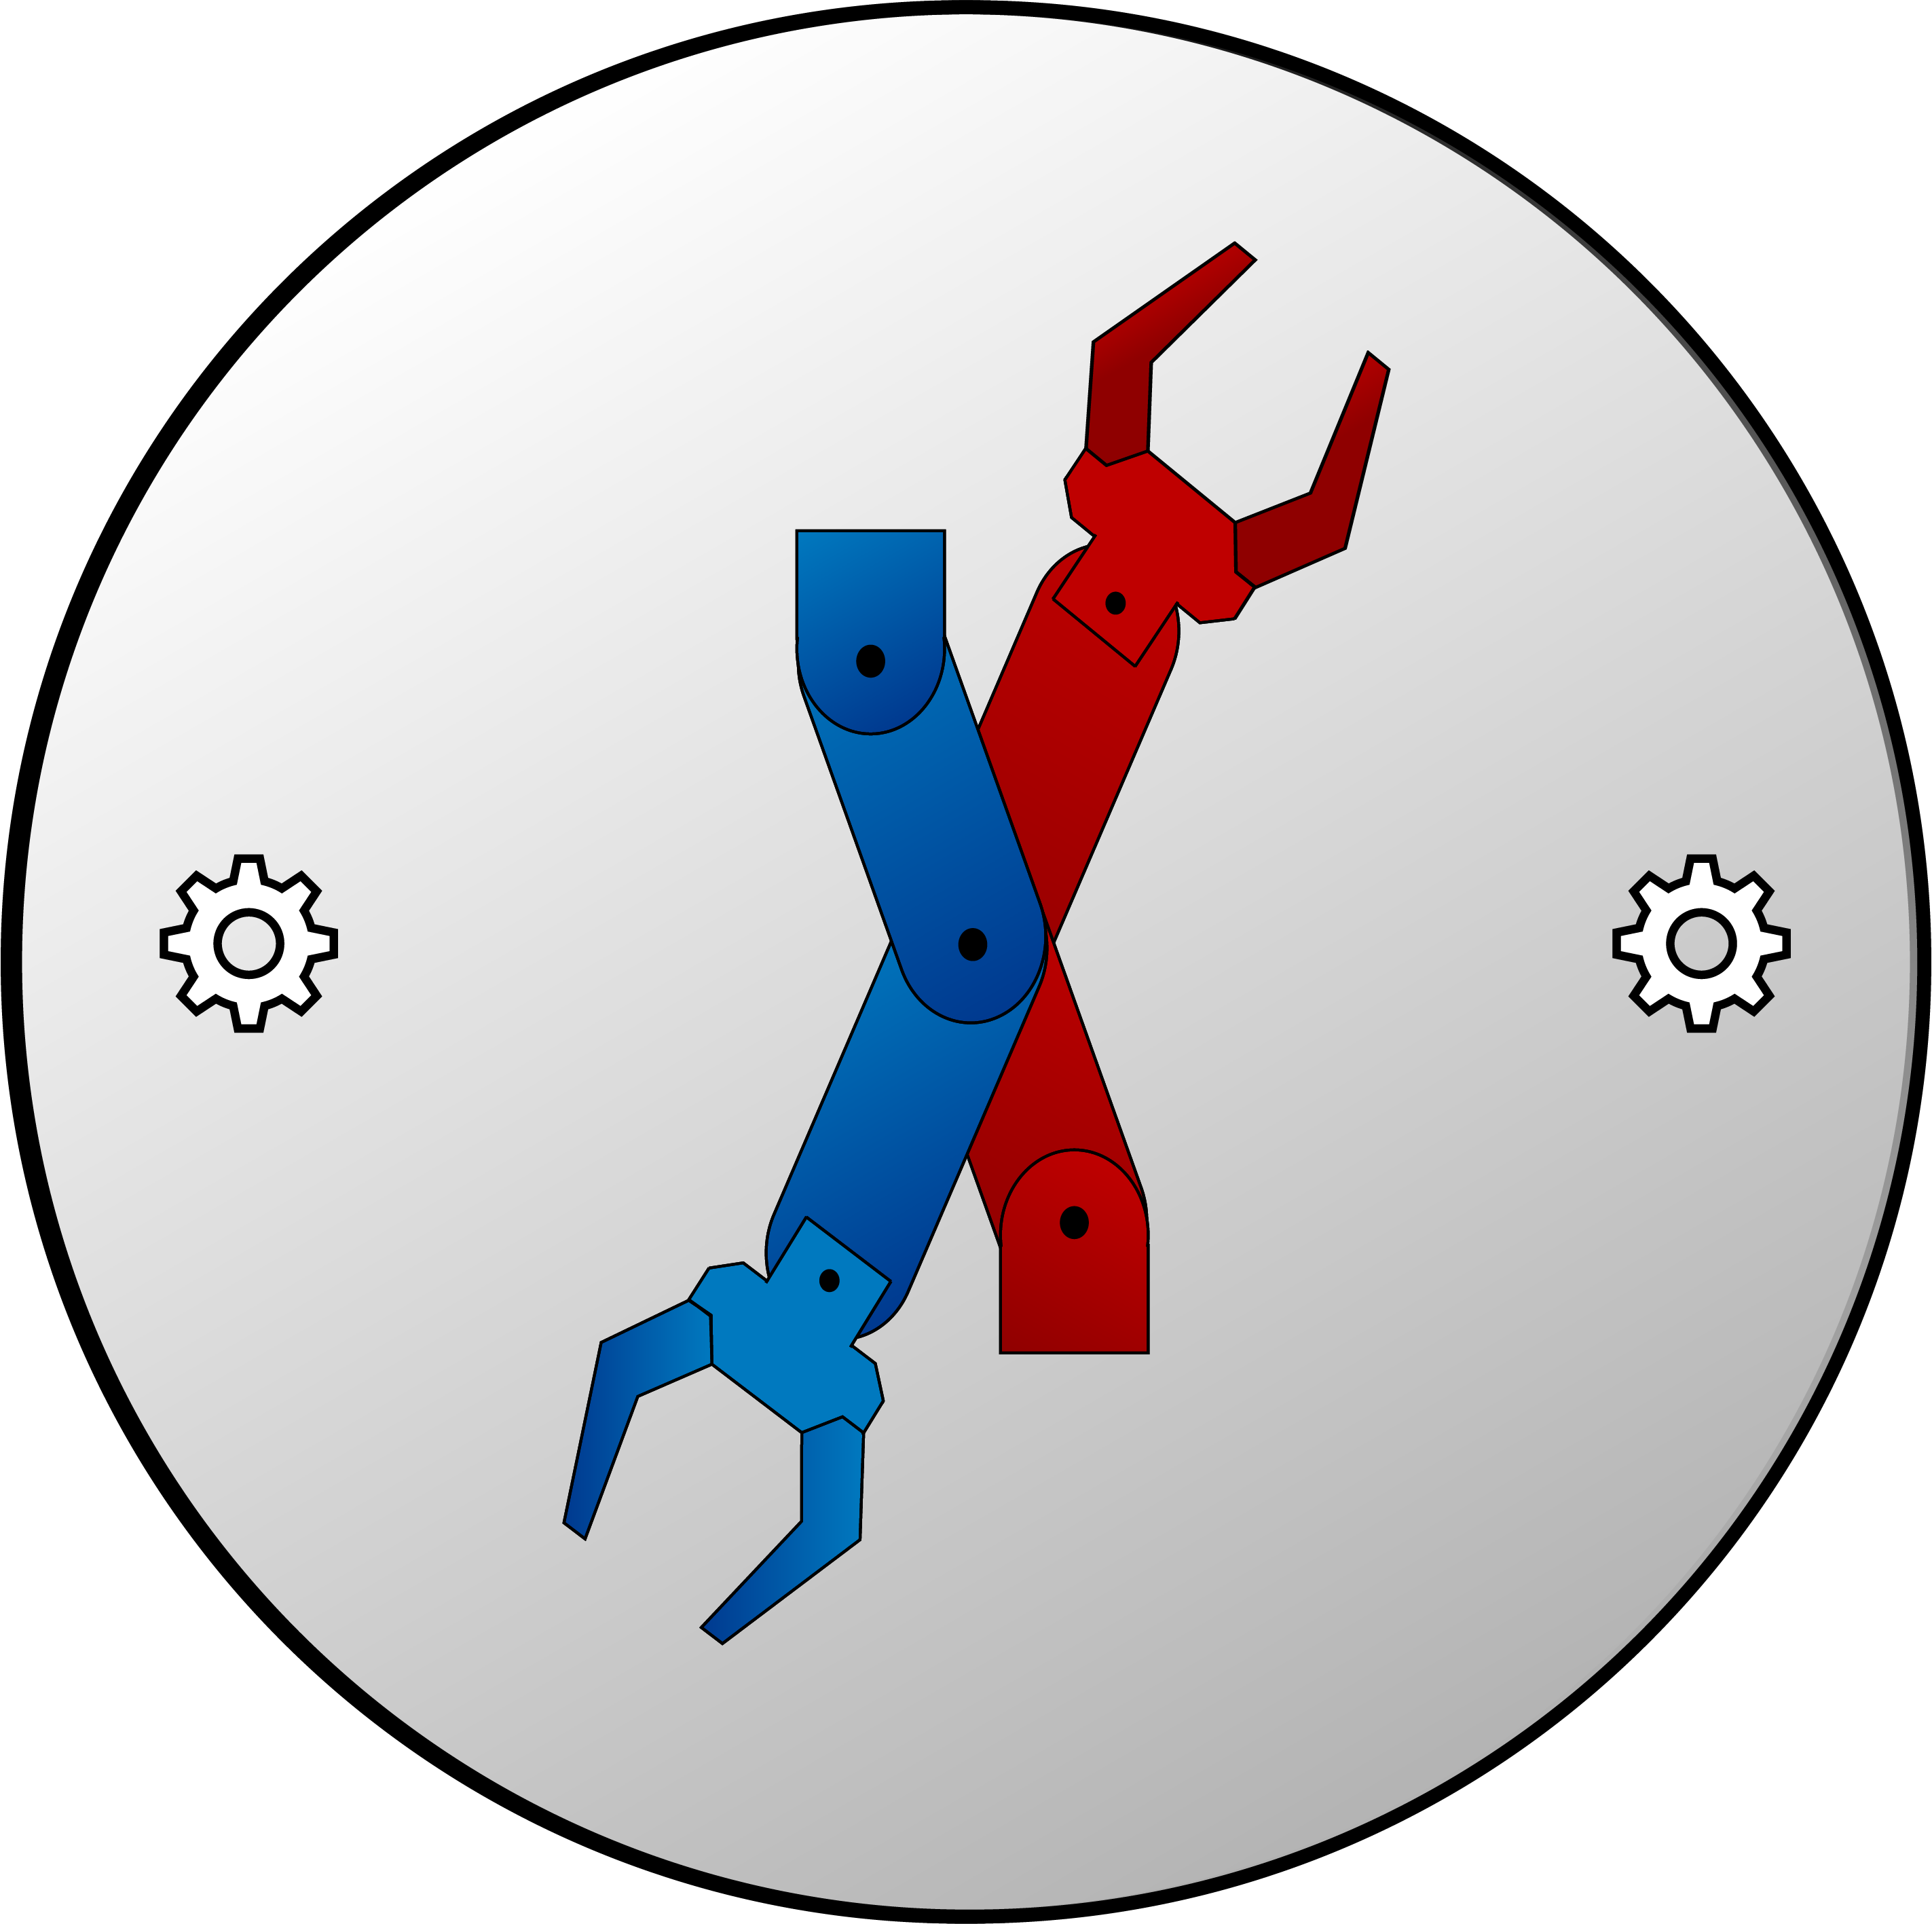
\includegraphics[width=.45\textwidth]{logo}
\vfill
\flushleft
ME 407 \\
Preliminary Design of Robotic Systems \\
Embry-Riddle Aeronautical University \\
\vspace{2ex}
\begin{minipage}[c]{.5\textwidth}
\flushleft

\includegraphics[width=.95\textwidth]{erau}
\end{minipage}%
\begin{minipage}[c]{.5\textwidth}
\flushright

\includegraphics[width=.8\textwidth]{text}
\end{minipage}
\end{titlepage}

\pagenumbering{roman}
% \begin{abstract}
  % Wordy words
% \end{abstract}
{\tableofcontents\let\clearpage\relax\listoffigures\listoftables}
\clearpage
\newpage
\pagenumbering{arabic}
\raggedright
\section{Introduction}\label{sec:intro}

With the intention of making robotics education more accessible to classrooms, the Manipulator for Educational Institutions with Open Source Integrated Systems (MEIOSIS) aims to provide robotics classes with an accurate and precise manipulator for cost lower than traditional manipulators. MEIOSIS is designed to be 3D printed by the end-user to reduce overall cost of the system and will be modifiable to create an increased understanding of robotics. The following document details the tests performed by the MEIOSIS team and the specific results obtained by each test. This is done in order to ensure that the design requirements are properly met by the finished product.


\section{Specifications and Tests}\label{sec:tests}
The goal of testing each individual specification is to acquire feedback in order to enhance the design of MEIOSIS. The Specifications and Tests section of the document overviews the tests done and the data/results acquired from the tests.

Specification \textbf{1.1.a} states: \textbf{The cost for the MEIOSIS team to develop the manipulator shall cost no more than \$800.} Team MEIOSIS meets this specification if the cost for the MEIOSIS team to develop the manipulator does not exceed \$800. This specification is tested by adding together the total cost of all parts ordered. This process can be seen in Table \ref{tab:bom}.

\begin{table}[htp]
  \centering
  \caption{MEIOSIS Bill of Materials with Costs}
  \label{tab:bom}
  \begin{tabular}{c|c|c|c}
  Product & Quantity & Individual Price & Transaction Cost \\\hline
  M3x30mm Screws & 2 & \$5.99 & \$11.98 \\
  M3 Locking nuts & 1 & \$7.99 & \$7.99 \\
  TRiREAK AC Bearing & 7 & \$9.00 & \$63.00 \\
  Dynamixel MX-12W & 3 & \$65.90 & \$197.70 \\
  Thrust Bearing & 1 & \$7.99 & \$7.99 \\
  Skateboard Bearings & 1 & \$5.29 & \$5.29 \\
  Pi 3 B & 1 & \$34.95 & \$34.95 \\
  Power Supply & 1 & \$9.95 & \$9.95 \\
  SD Card & 1 & \$12.95 & \$12.95 \\
  Shipping/Tax & 1 & N/A & \$7.95 \\
  Discounts & 1 & N/A & -\$8.17 \\
  &&&\\
  & & \textbf{Total Cost} & \$351.58 \\
  \end{tabular}
\end{table}

In Table 1, the “Shipping/Tax” row shows the listed shipping fees for the Pi 3 B and associated parts. The “Discounts” row shows the sum total of all the small discounts that were applied to the bulk purchases of multiple items. Table 1 also demonstrates that the total cost to develop the manipulator was \$351.58, well under the \$800 allocated for this project, signifying that \textbf{Specification 1.1.a was met by the product.}


Specification \textbf{1.2.a} states: \textbf{The system shall consist of six rotational joints connected by four links. The last three joints will create a spherical wrist.} For this specification to be met, the robot must have six rotational joints and four links. The last three joints must create a spherical wrist where the axis of revolution for the last three joints are intersecting with one another. To perform a test to check for six rotational joints, SolidWorks is required. A rendering of the manipulator with labeled joints can be seen in Figure \ref{fig:manip}.


\begin{figure}[htp]
  \centering
  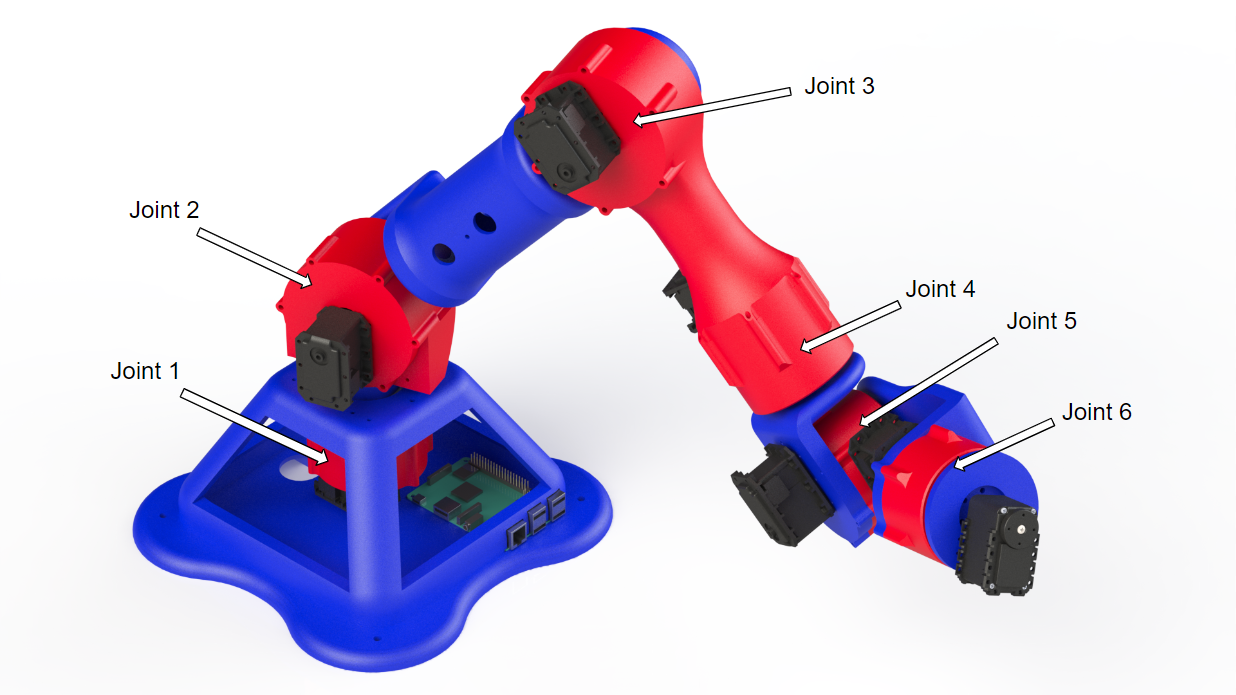
\includegraphics[width=.75\textwidth,frame]{manip}
  \caption{Labeled Image of Manipulator Rendering}
  \label{fig:manip}
\end{figure}

As is illustrated in Figure 1, the robot consists of six rotational joints. Joint 1 controls the rotation about the base,  joints 2 and 3 control the “shoulder” and “elbow” of the robot, and joints 4, 5, and 6 control the  spherical wrist. The rotational axis of joint 4 intersects with joint 5’s and joint 5’s intersects with joint 6’s rotational axis. To perform this test, the assembly file containing the manipulator was opened and the joints were counted. Using the move tool, each joint can be observed to be exclusively rotational. The data obtained is simulated due to the fact that the robot has not been fully fabricated. \textbf{This manipulator meets specification 1.2.a}.

\newpage
Specification \textbf{1.2.b} states: \textbf{The system shall have no link offsets.} For this specification to be satisfied, there must be no link offsets present in the design of the robotic manipulator meaning that the link should connect two joints by translating in only one direction and the axes of the joints attached to the link should be collinear with one another. Testing this specification requires SolidWorks’ measurement tool. Using the measurement tool, measure each joint to ensure there is only displacement along one axis. Figure \ref{fig:loff} shows an example of a measurement done on the elbow link of the manipulator.

\begin{figure}[htp]
  \centering
  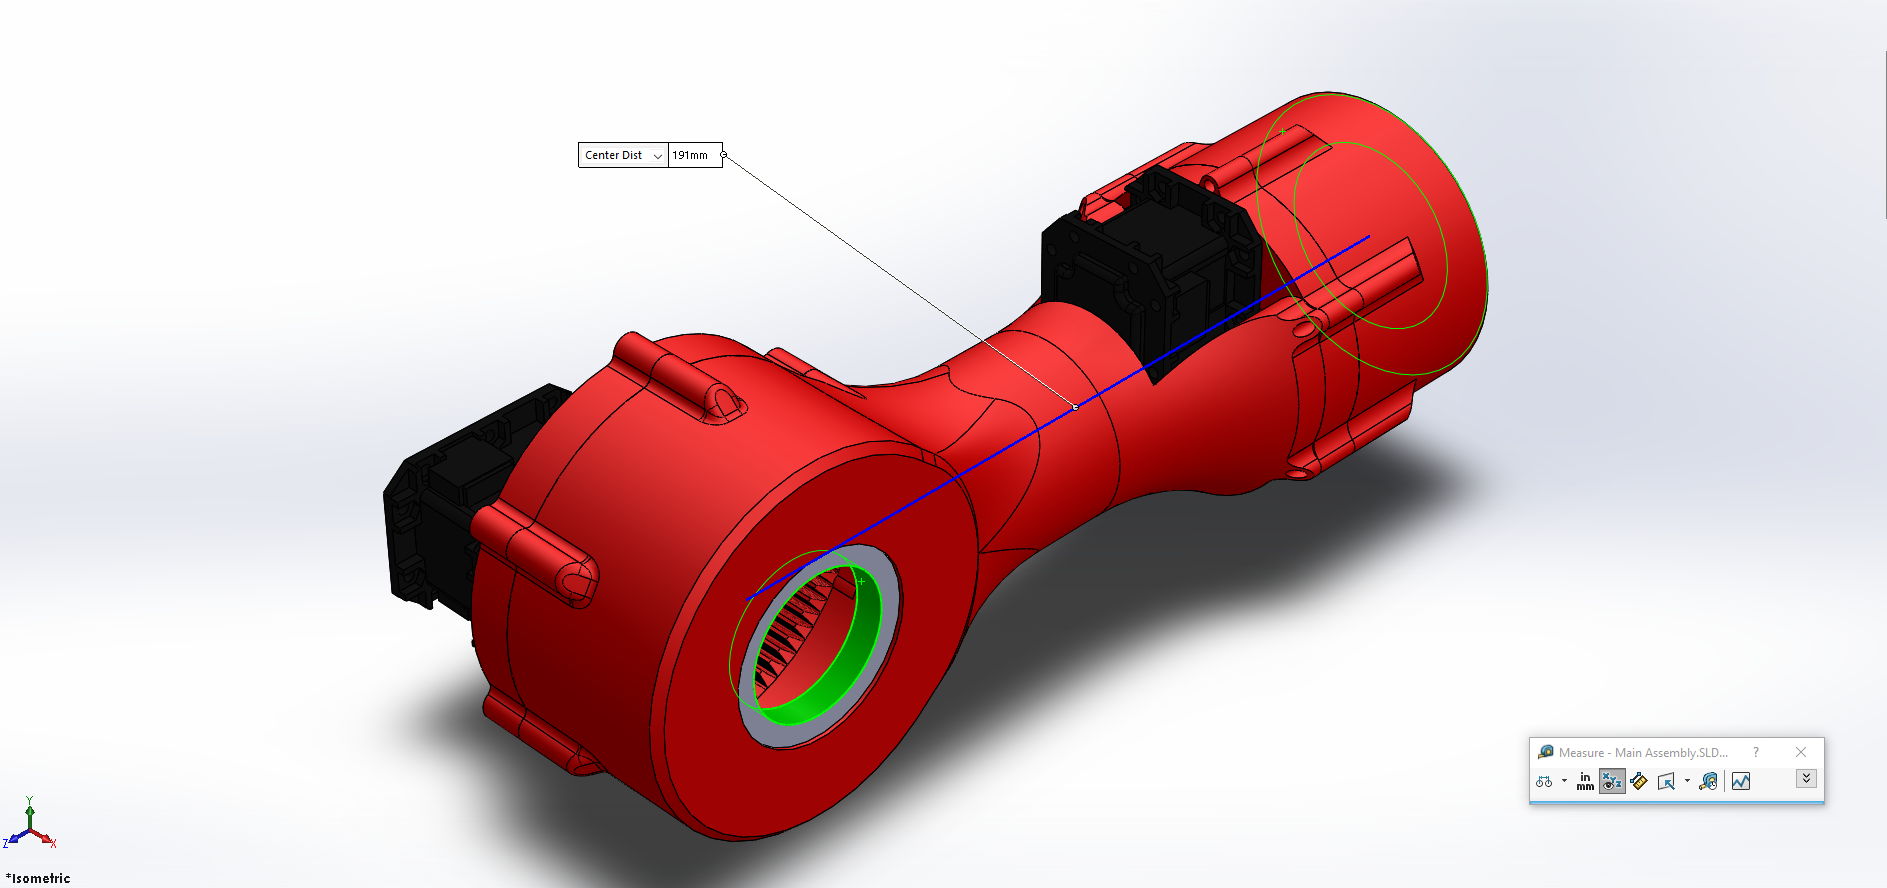
\includegraphics[width=.75\textwidth,frame]{loff}
  \caption{Measurement Test for Link Offset}
  \label{fig:loff}
\end{figure}

Figure \ref{fig:loff} shows a screen capture of a measurement taken. The blue line, the link only extends across one axis and if there were a link offset present, there would be multiple multi-colored lines to show displacement in multiple directions. These tests were done in simulation on each link of the manipulator and none contained any offset direction. Through this test, it is observed that \textbf{the manipulator meets specification 1.2.b}.

Specification \textbf{1.3.a} states: \textbf{The system shall accommodate a process in which the end user can calibrate the end effector position and orientation to within 0.5 mm and 1 degree of the manipulator’s precision.} In order to fulfill specification 1.3.a, an algorithm was developed for calibration. This algorithm must allow the user to manually move the links into a desired zeroed configuration, then accurately retain that zeroed configuration as a reference position during use. Figure \ref{fig:zero} depicts the manipulator in a zeroed configuration.

\newpage
\begin{figure}[htp]
  \centering
  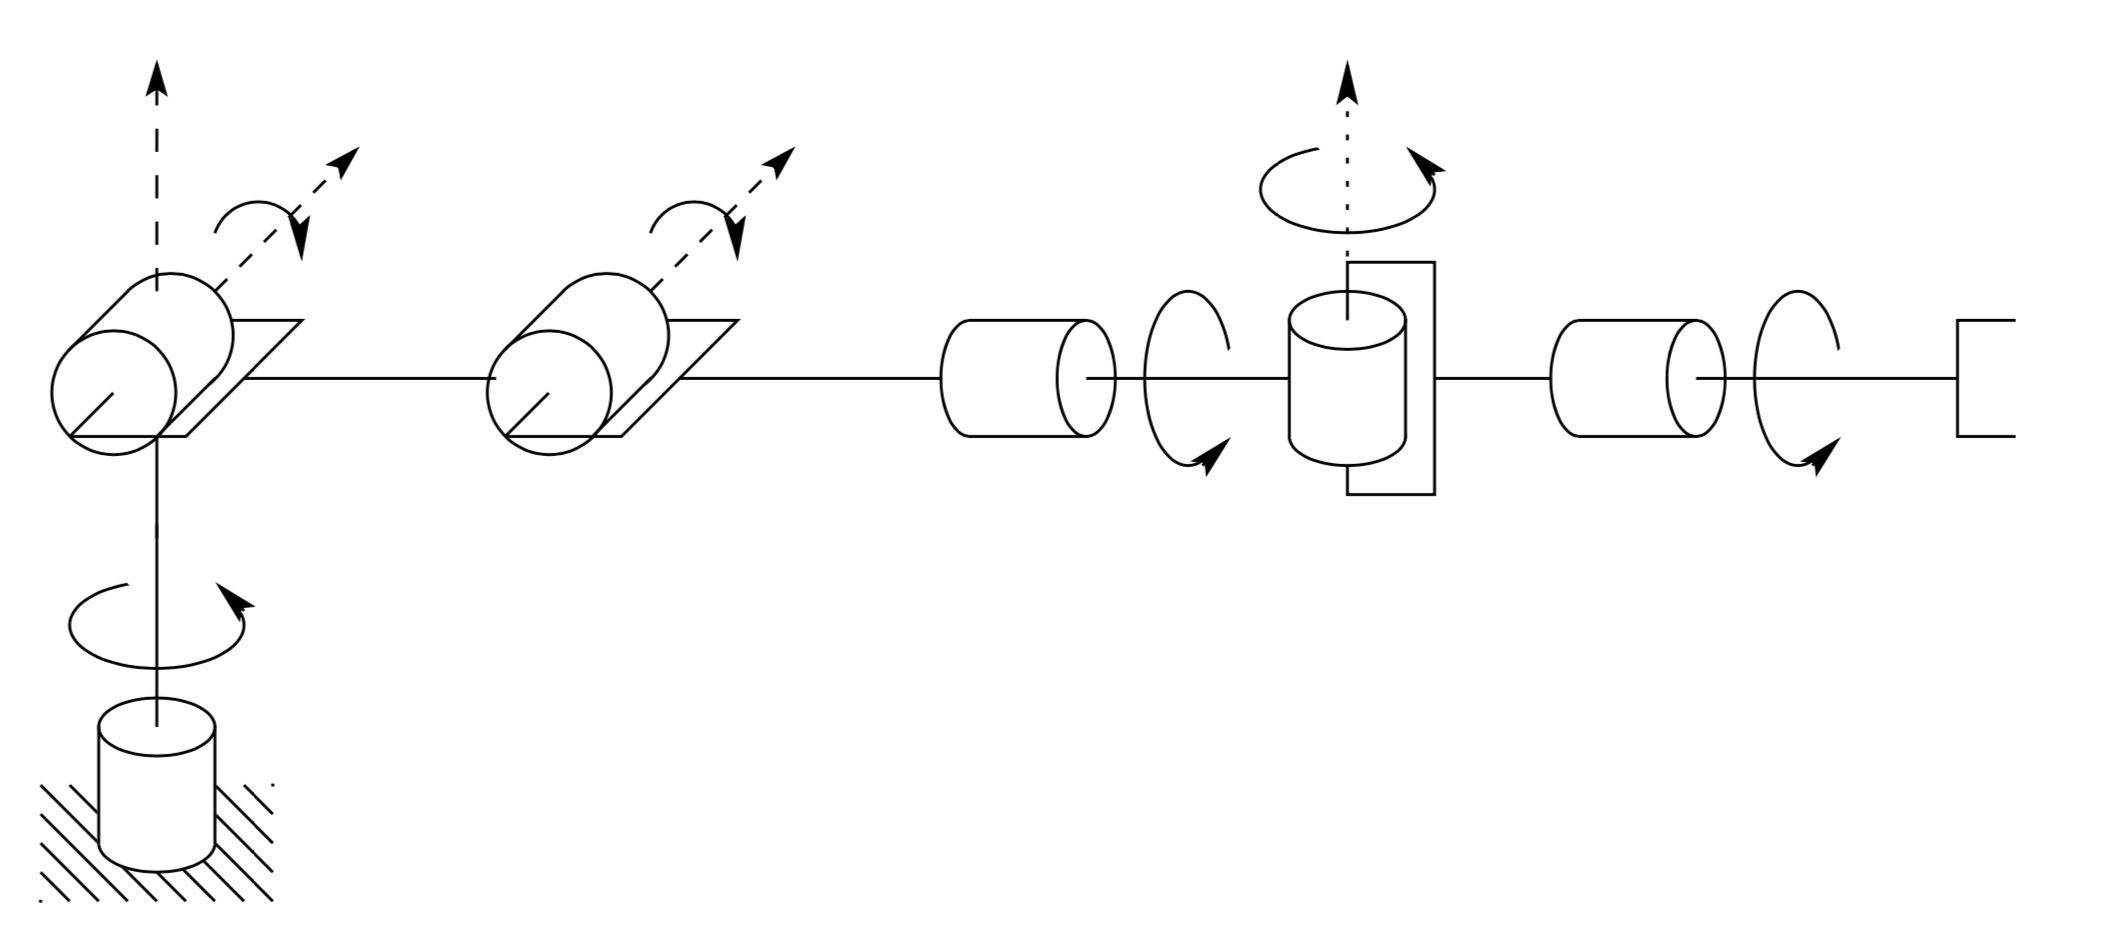
\includegraphics[width=.75\textwidth,frame]{zero}
  \caption{Manipulator in its Zeroed Configuration}
  \label{fig:zero}
\end{figure}

The configuration shown in Figure \ref{fig:zero} is what we have defined to be the zeroed configuration. The purpose of the calibration algorithm is to force the software to consider every joint angle to be zero when the manipulator is in this configuration, even if the servos return non-zero angular values. The algorithm developed allows the users to move the joints one by one until the robot is in the desired “zeroed” position. The program then reads the servos positions and stores those values as offset variables. These offsets are subtracted from the desired joint angle values when commanding the servo positions.

In order to measure the calibration accuracy, the PhaseSpace Motion Capture system will be required. The calibration algorithm itself is accurate to the same value as the manipulator, however inaccuracies can arise due to the user not being able to manually put the manipulator into the correct configuration. In completing this testing procedure, it is assumed that the motion capture system will be fully set up, including placing the tracking markers on the manipulator’s base and end-effector. Once the motion capture system is fully set up, the manipulator will be placed in an arbitrary configuration, at least 30° away from zero in each joint. The manipulator will then be restarted, which will erase the system’s memory of it’s configuration. At this point, the motion capture system will start recording data. Using the calibration software, the manipulator will then be manually zeroed to the best of the operator’s abilities. Once the zeroing is completed, error terms can be determined by comparing the tracking data to the known values of the end-effector’s position and orientation in the zeroed state. Due to circumstances beyond our control, we are not able to perform this test and \textbf{adherence to specification 1.3.a cannot be determined.}

\newpage
Specification \textbf{1.4.a} states: \textbf{Joint one and two of the system shall possess an angle error of no more than 0.025 degrees.} Specification \textbf{1.4.b} states: \textbf{Joint three of the system shall possess an angle error of no more than .03 degrees.} Specification \textbf{1.4.c} states: \textbf{Joints four, five, and six shall possess an angle error of no more than .29 degrees.} In order to verify specifications 1.4.a, 1.4.b, and 1.4.c, the angle accuracy of the system must be measured. To determine the accuracy, the PhaseSpace Motion Capture System is required. Three LED indicators will be placed at the end of each gearbox that is farthest from the previous gearbox in the line to indicate the farthest point directly controlled by the previous gearbox. The three LEDs will be placed at 120° increments around each link/gearbox so that one or more of the LEDs are visible to the motion capture system at a time. To attain accurate results, small divots will be placed on the manipulator where the LEDs will be located which allows for precise application of the LEDs to the system. Accurate LED placement will allow for more accurate kinematic/angle calculations.

To test the system, the manipulator will be placed in the zeroed configuration and each joint will be tested individually. First, joint 1 will be tested by running from 0° to 90°, and then back to 0° ten times. Each time joint 1 has reached 90°, the motion capture system will collect the location data of the LEDs and store it for error calculation. When this procedure is completed, the data can be used to calculate the angle the link actually achieved, and can be compared to the desired angle. Any error in zeroing will be seen from the collected data. After joint 1 has been tested, joint 2 will be tested following the same procedure, after which joints 3 through 6 will be tested in order. The worst angle error achieved by each joint will be compared to the value defined in the specifications. This test is unable to be performed without lab access and thus \textbf{the manipulator’s adherence to specifications 1.4a-1.4c cannot be determined.}


Specification \textbf{1.5.a} states: \textbf{The manipulator shall have a maximum reach between 300 and 700 mm.} In order to satisfy this specification, the robot’s links must have a sum length of between 300 mm and 700 mm. Using Solidworks, the total reachable workspace can be measured using the “Measure” tool. This measurement can be seen in Figure \ref{fig:meas}.

\newpage
\begin{figure}[htp]
  \centering
  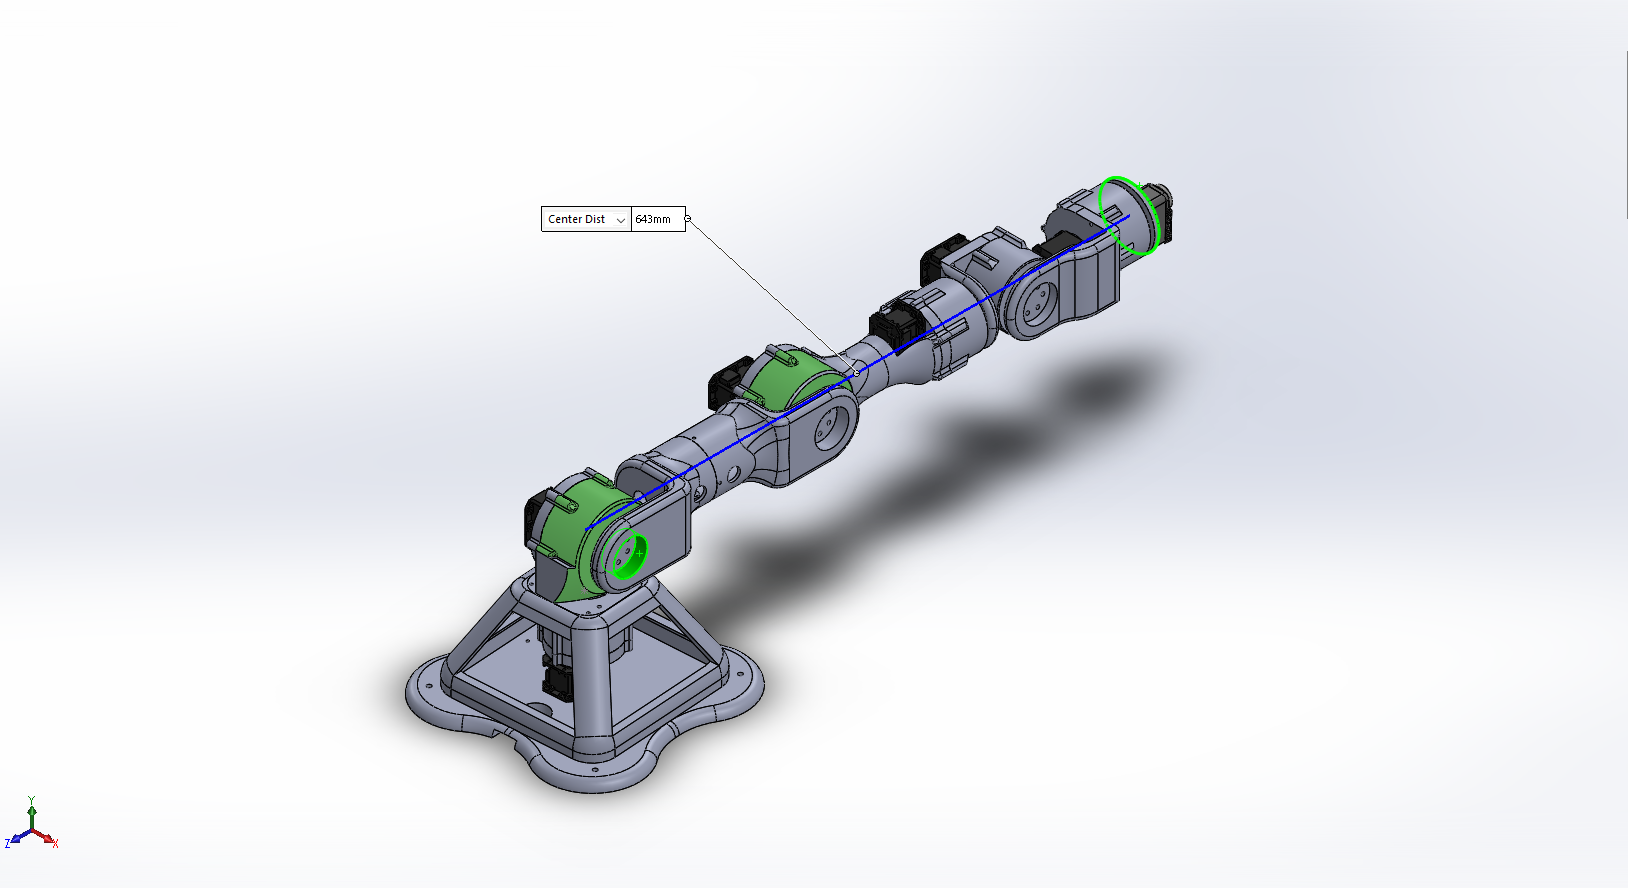
\includegraphics[width=.75\textwidth,frame]{image8}
  \caption{Solidworks Measurement of Reachable Workspace}
  \label{fig:meas}
\end{figure}

As can be seen in Figure \ref{fig:meas}, the total reachable workspace is 643 mm. This measurement is between 300 and 700 millimeters and therefore \textbf{the manipulator meets specification 1.5.a.}

Specification \textbf{1.5.b} states: \textbf{The length of links one, two, three, and the wrist shall be 161.5 mm, 250 mm, 250 mm, and 143 mm respectively.} For the manipulator to meet specification 1.5.a, each link and the wrist simply need to match the lengths provided in the specification. Testing this specification requires the SolidWorks measurement tool. An example of the measurement tool being used to test this specification can be seen in Figure \ref{fig:llength}.

\begin{figure}[htp]
  \centering
  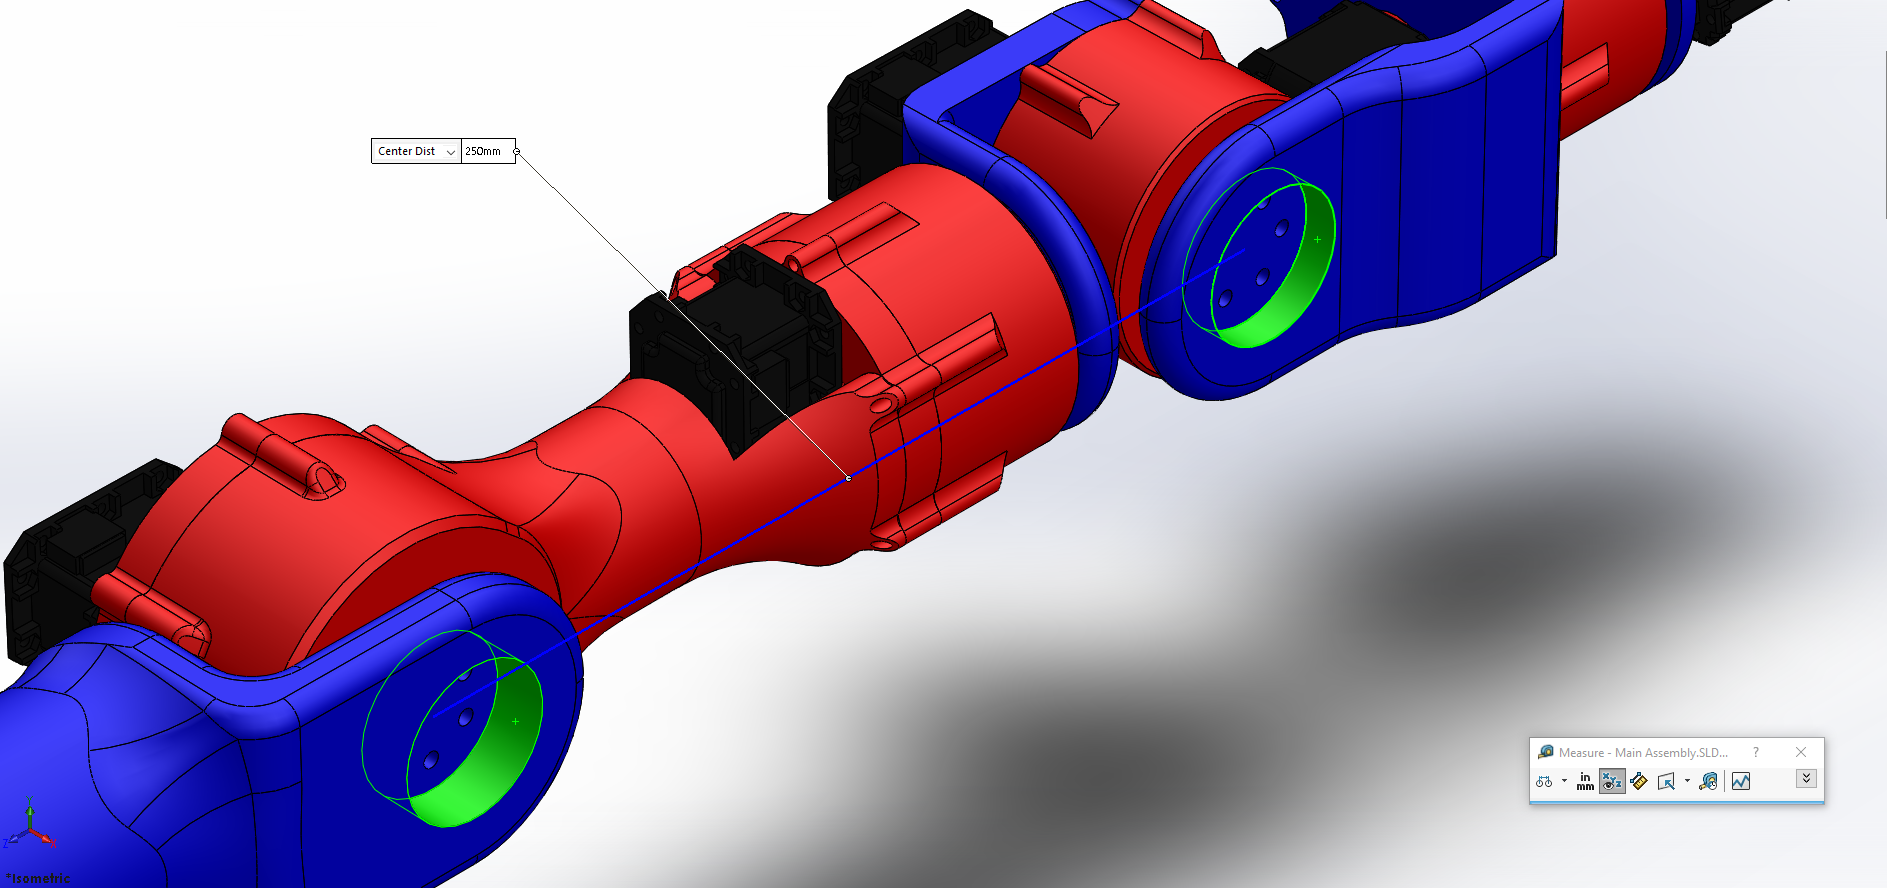
\includegraphics[width=.75\textwidth,frame]{image11}
  \caption{Test of Link Length for Specification 1.5.a.}
  \label{fig:llength}
\end{figure}

Once the measurement tool in SolidWorks is selected, a measurement from the first joint in a link to the last joint in a link should be taken. Figure \ref{fig:llength} shows a measurement between joints 3 and 5, these joints make up Link 3 or the “elbow” link of the manipulator. The center distance measurement came out to be 250 mm. Once a measurement is done for each link, the center distance values are to be recorded. The variable factors in these measurements are the dimensions of the parts used to make up the link lengths. The lengths of the individual links can be seen in Table \ref{tab:linklengths}. These dimensions are simulated in SolidWorks.

\begin{table}[htp]
  \centering
  \caption{Measurements of Manipulator Link Lengths}
  \label{tab:linklengths}
  \begin{tabular}{c|c}
    Portion of manipulator measured & Measurement Value \\\hline
    Link 1 (Base to Joint 2) & 161.5 mm \\
    Link 2 (Joint 2 to Joint 3) & 250 mm \\
    Link 3 (Joint 3 to Joint 5) & 250 mm \\
    Wrist (Joint 5 to End Effector) & 143 mm \\
  \end{tabular}
\end{table}

As can be seen by Table \ref{tab:linklengths}, the link measurements obtained in SolidWorks match the measurements provided by specification 1.5.a and the \textbf{manipulator meets the specification. }


Specification \textbf{1.6.a} states: \textbf{The system’s workspace must contain a hemispherical shell that has a thickness of 280 mm where the robot is theoretically fully dexterous.} In order to test the dexterity of the manipulator and ensure that it fulfills specification 1.6.a, a program was created that tests a series of points for dexterity. These points are 1 mm apart to match the manipulator’s precision and can be rotated around the z-axis to create a hemispherical shell. The script accomplishes this by calculating the inverse kinematics for the manipulator, given its dimensions. If any point is outside of the manipulator’s workspace it is marked on a MATLAB plot, as can be seen in Figure \ref{fig:plot1}.

\let\clearpage\relax
\begin{figure}[htp]
  \centering
  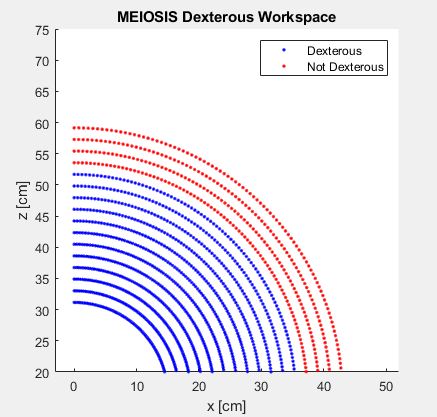
\includegraphics[width=0.5\textwidth,frame]{workspace}
  \caption{Matlab Plot of Invalid Dexterity Check}
  \label{fig:plot1}
\end{figure}

Figure \ref{fig:plot1} shows a failed configuration for our dexterity check. At approximately 35 cm away from the robot it is no longer fully dexterous in this configuration. In order to fix this, changes to the design need to be made, specifically the length of the links. Another fix would be moving the dexterous workspace closer to the base of the robot, however it cannot be moved too close since the base of the robot would be in the way. Figure \ref{fig:plot2} shows a successful dexterity check.

\begin{figure}[htp]
  \centering
  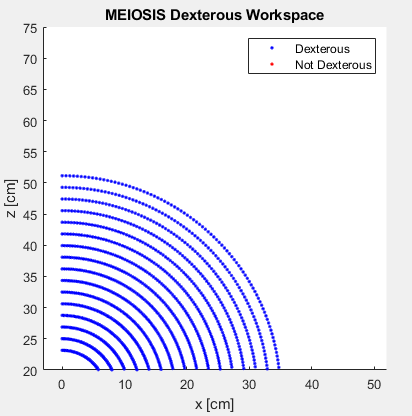
\includegraphics[width=0.5\textwidth,frame]{image4}
  \caption{Matlab Plot of Successful Dexterity Check}
  \label{fig:plot2}
\end{figure}

As can be seen in Figure \ref{fig:plot2}, a successful dexterity check was achieved and the requirement is met. The dexterous workspace spans from 70 mm away from the base to 350 mm away from the base and thus creates a hemispherical workspace with a thickness of 280 mm, thus \textbf{the manipulator fulfills specification 1.6.a.}


Specification \textbf{1.6.b} states: \textbf{The rotational limit of joint one, two, three, four, five, and six shall be -165° to 180°, 13.7° to 179.8°, -179.6° to -19.2°, ±180°, -180° to 0°, and ±180° respectively.} This specification is met if the links can rotate to the maximum and minimum angles provided by the specification. These angles were tested in SolidWorks using the measurement tool. The links to be measured are moved until they collide with one another and then the measurement tool is selected. Once the measurement tool is selected, the two links that form the angle to be measured are selected and the “create sensor” button is pressed. SolidWorks then provides the angle in degrees on the left sidebar. The angles for each joint are then recorded and the results of the measurements can be seen in Table \ref{tab:table2}.

\newpage
\begin{table}[htp]
  \centering
  \caption{Results of Angle Measurement Test for Specification 2.1.6.a}
  \label{tab:table2}
  \begin{tabular}{c|c|c|c}
    Joint Number & Minimum Angle & Maximum Angle & Specification Met? \\\hline
    1 & -180° & 180° & \cmark \\
    2 & -21° & 201° & \cmark \\
    3 & -126° & 126° & \xmark \\
    4 & -180° & 180° & \cmark \\
    5 & -75° & 115° & \xmark \\
    6 & -180° & 180° & \cmark \\
  \end{tabular}
\end{table}

Table \ref{tab:table2} shows that the measurements for joints 3 and 5 do not meet the specification’s individual requirements for them, therefore \textbf{the manipulator does not meet specification 1.6.b.} This specification could be met following a major redesign of the system’s link and joint system.


Specification \textbf{1.7a} states: \textbf{The system shall use a parallel gripper that can close to 18 mm.} To meet specification 1.7.a, a parallel gripper must be designed or purchased that can close to a distance of 18 mm or smaller. Dynamixel offers a parallel gripper actuated by an AX-12A servo as shown in Figure \ref{fig:gripper1}. This gripper can be utilized since the manipulator’s end effector is designed to attach an AX-12A smart servo.

\begin{figure}[htp]
  \centering
  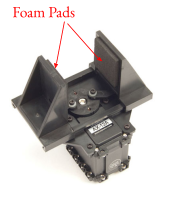
\includegraphics[width=0.3\textwidth,frame]{image10}
  \caption{Dynamixel Parallel Gripper with Servo \cite{gripper1}}
  \label{fig:gripper1}
\end{figure}

As depicted in Figure \ref{fig:gripper1}, the gripper is open to its widest extent. However, the gripper’s fingers have removable foam pads. The foam pads allow adjustments in the gripping plasticity and the maximum opening/closure. Figure \ref{fig:gripper2} shows the gripper in various configurations.
\newpage
\begin{figure}[ht]
  \centering
  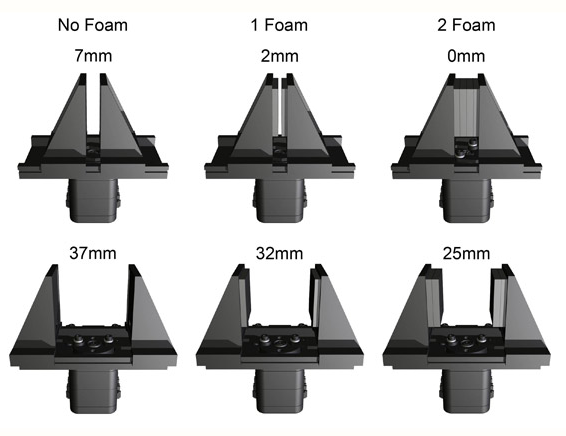
\includegraphics[width=0.6\textwidth,frame]{image9}
  \caption{Dynamixel Gripper with and without Foam Padding at Minimum and Maximum Opening \cite{gripper1}}
  \label{fig:gripper2}
\end{figure}

The top three gripper configurations, shown in Figure \ref{fig:gripper2}, are fully closed and the bottom three are fully opened. From left to right, the fingers have no, one, and two pieces of foam. The maximum opening with no foam is 37 mm and the maximum closure is 0 mm with four pieces of foam. While none of these configurations have exactly 18 mm between the fingers the distance between the fingers can be adjusted to accommodate this, as shown in Figure \ref{fig:gripper3}.

\begin{figure}[htp]
  \centering
  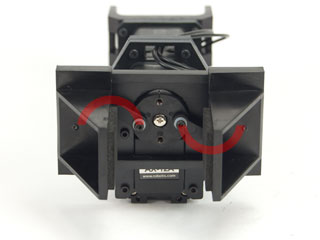
\includegraphics[width=0.5\textwidth,frame]{image3}
  \caption{Dynamixel Gripper Rotational to Linear Motion Mechanism \cite{gripper2}}
  \label{fig:gripper3}
\end{figure}

By sending the servo a position, the two highlighted red half-circular bars seen in Figure \ref{fig:gripper3} pivot about the servo face’s edges, translating the fingers either inward or outward. Clockwise rotation would decrease the distance between the fingers, while counterclockwise rotation would increase the distance. The closure’s precision would be dictated by the AX-12A’s resolution. Since the precision of the 18mm closing distance is not specified, it can be assumed the precion need only be sufficient to prevent the marker from being dislodged during writing, which is addressed in 1.8.a. Therefore, no matter the number of foam pads applied, the gripper can close to 18 mm. With the Dynamixel Parallel gripper being used as an end effector attachment, \textbf{the manipulator meets specification 1.7.a.}


Specification \textbf{1.7.b} states: \textbf{The end effector shall attach to the manipulator using screws configured in a pattern that can accommodate a Dynamixel AX-12A servo.} In order to meet this specification, a dynamixel AX-12A smart servo must be compatible with the end effector’s screw configuration. This can simply be tested using screws and a screwdriver. If the smart servo can successfully be screwed onto the end effector, then this specification is met. The design matches measurements acquired in the lab and parts to accommodate an AX-12A were fabricated and assembled in the lab. Since the dynamixel smart servos have been tested and observed to fit on the parts printed, \textbf{the manipulator meets specification 1.7.b}.


Specification \textbf{1.8.a} states: \textbf{The gripper shall be able to support 0.004 Newton meter moments about the axes normal to its gripping surfaces.} To meet specification 1.8.a, the gripper selected to be attached to the manipulator’s end effector should be capable of holding an object that provides 0.004 Newton meter moments about the axes normal to its gripping surfaces. Using the same Dynamixel gripper seen in Figure \ref{fig:gripper4}, a test can be performed

\begin{figure}[htp]
  \centering
  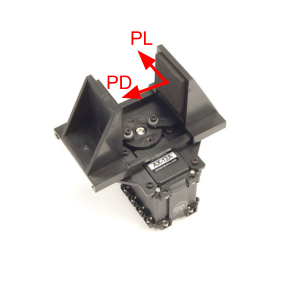
\includegraphics[width=0.3\textwidth,frame]{image12}
  \caption{Dynamixel Parallel Gripper with Servo \cite{gripper1}}
  \label{fig:gripper4}
\end{figure}

For testing, we can consider the convenient coordinate frame shown in Figure \ref{fig:gripper4}. Specifically, when writing, moments caused by the Expo marker’s contact force with paper can be decomposed along the axes of this coordinate frame. In the best case scenario, the marker provides force parallel to and perpendicular to the gripping plane denoted by PL and PD respectively.
To test this specification, a set of masses and an Expo marker  are required. First, the servo would be commanded to close the gripper on the Expo marker and the masses would be gradually hung from the end of the Expo marker. The moment could be calculated as more mass is added. If the marker is observed to slip or rotate, the moment is too large for the gripper. The gripper would be tested at different angles, grip force, and number of pieces of foam attached, as can be seen in Figure 7. Due to unforeseen circumstances, \textbf{adherence to specification 1.8.a cannot be determined.}


Specification \textbf{2.1.a} states: \textbf{The software shall be hosted publicly on an online repository and maintain an MIT license for distribution.} To satisfy this requirement, the software used to control the robot must be open source and publicly accessible. The use of the code repository GitHub allows team MEIOSIS to easily make the code publicly accessible; by using the MIT licensing, the software can be considered open source and possible legal implications due to misuse can be avoided. The license allows the end-user to modify, redistribute, or do whatever they please with the code: “...without limitation the rights to use, copy, modify, merge, publish, distribute, sublicense, and/or sell copies of the Software...”\cite{mit} The MIT license makes it such that any end-user that makes a system with the manipulator, i.e. repurposes the given system for a task, has no limitations with how they wish to redistribute, share, or even sell the system. To implement the use of the license, the source code must contain the proper header, shown by MIT \cite{mit}. The header was added and can be observed in the software as well as the code is hosted in a public GitHub repository. Therefore \textbf{the system fulfills specification 2.1.a.}


Specification \textbf{2.2.a} states: \textbf{The system shall have a user interface capable of accepting the end-effector’s desired cartesian position and Euler angle orientation as a six element row vector.} In order to satisfy specification 2.2.a, python scripts have been methodically developed to allow for user input of desired end effector position. These scripts could potentially be used as a backend for a graphical user interface (GUI) to further simplify the process of controlling the manipulator.

In lieu of a Python based GUI directly controlling the manipulator, a GUI could be created to instead control an animated simulation of the manipulator. The simulation is currently generated by a MATLAB script that draws the robot STL files into a figure window. The possibilities of controlling the simulation consist of several options, the most efficient would likely be to develop a user interface entirely with MATLAB. This GUI avoids possible incompatibilities on systems without Python installed and avoids any communication issues that could incur with attempting to create the GUI in another language.

\newpage
The best option is to have a MATLAB GUI control the MATLAB simulation, therefore a basic interface shall be created in which the user can select which control scheme is desired as well as goal positions for the end effector. A sample GUI can be seen in Figure \ref{fig:gui}.

\let\clearpage\relax
\begin{figure}[htp]
  \centering
  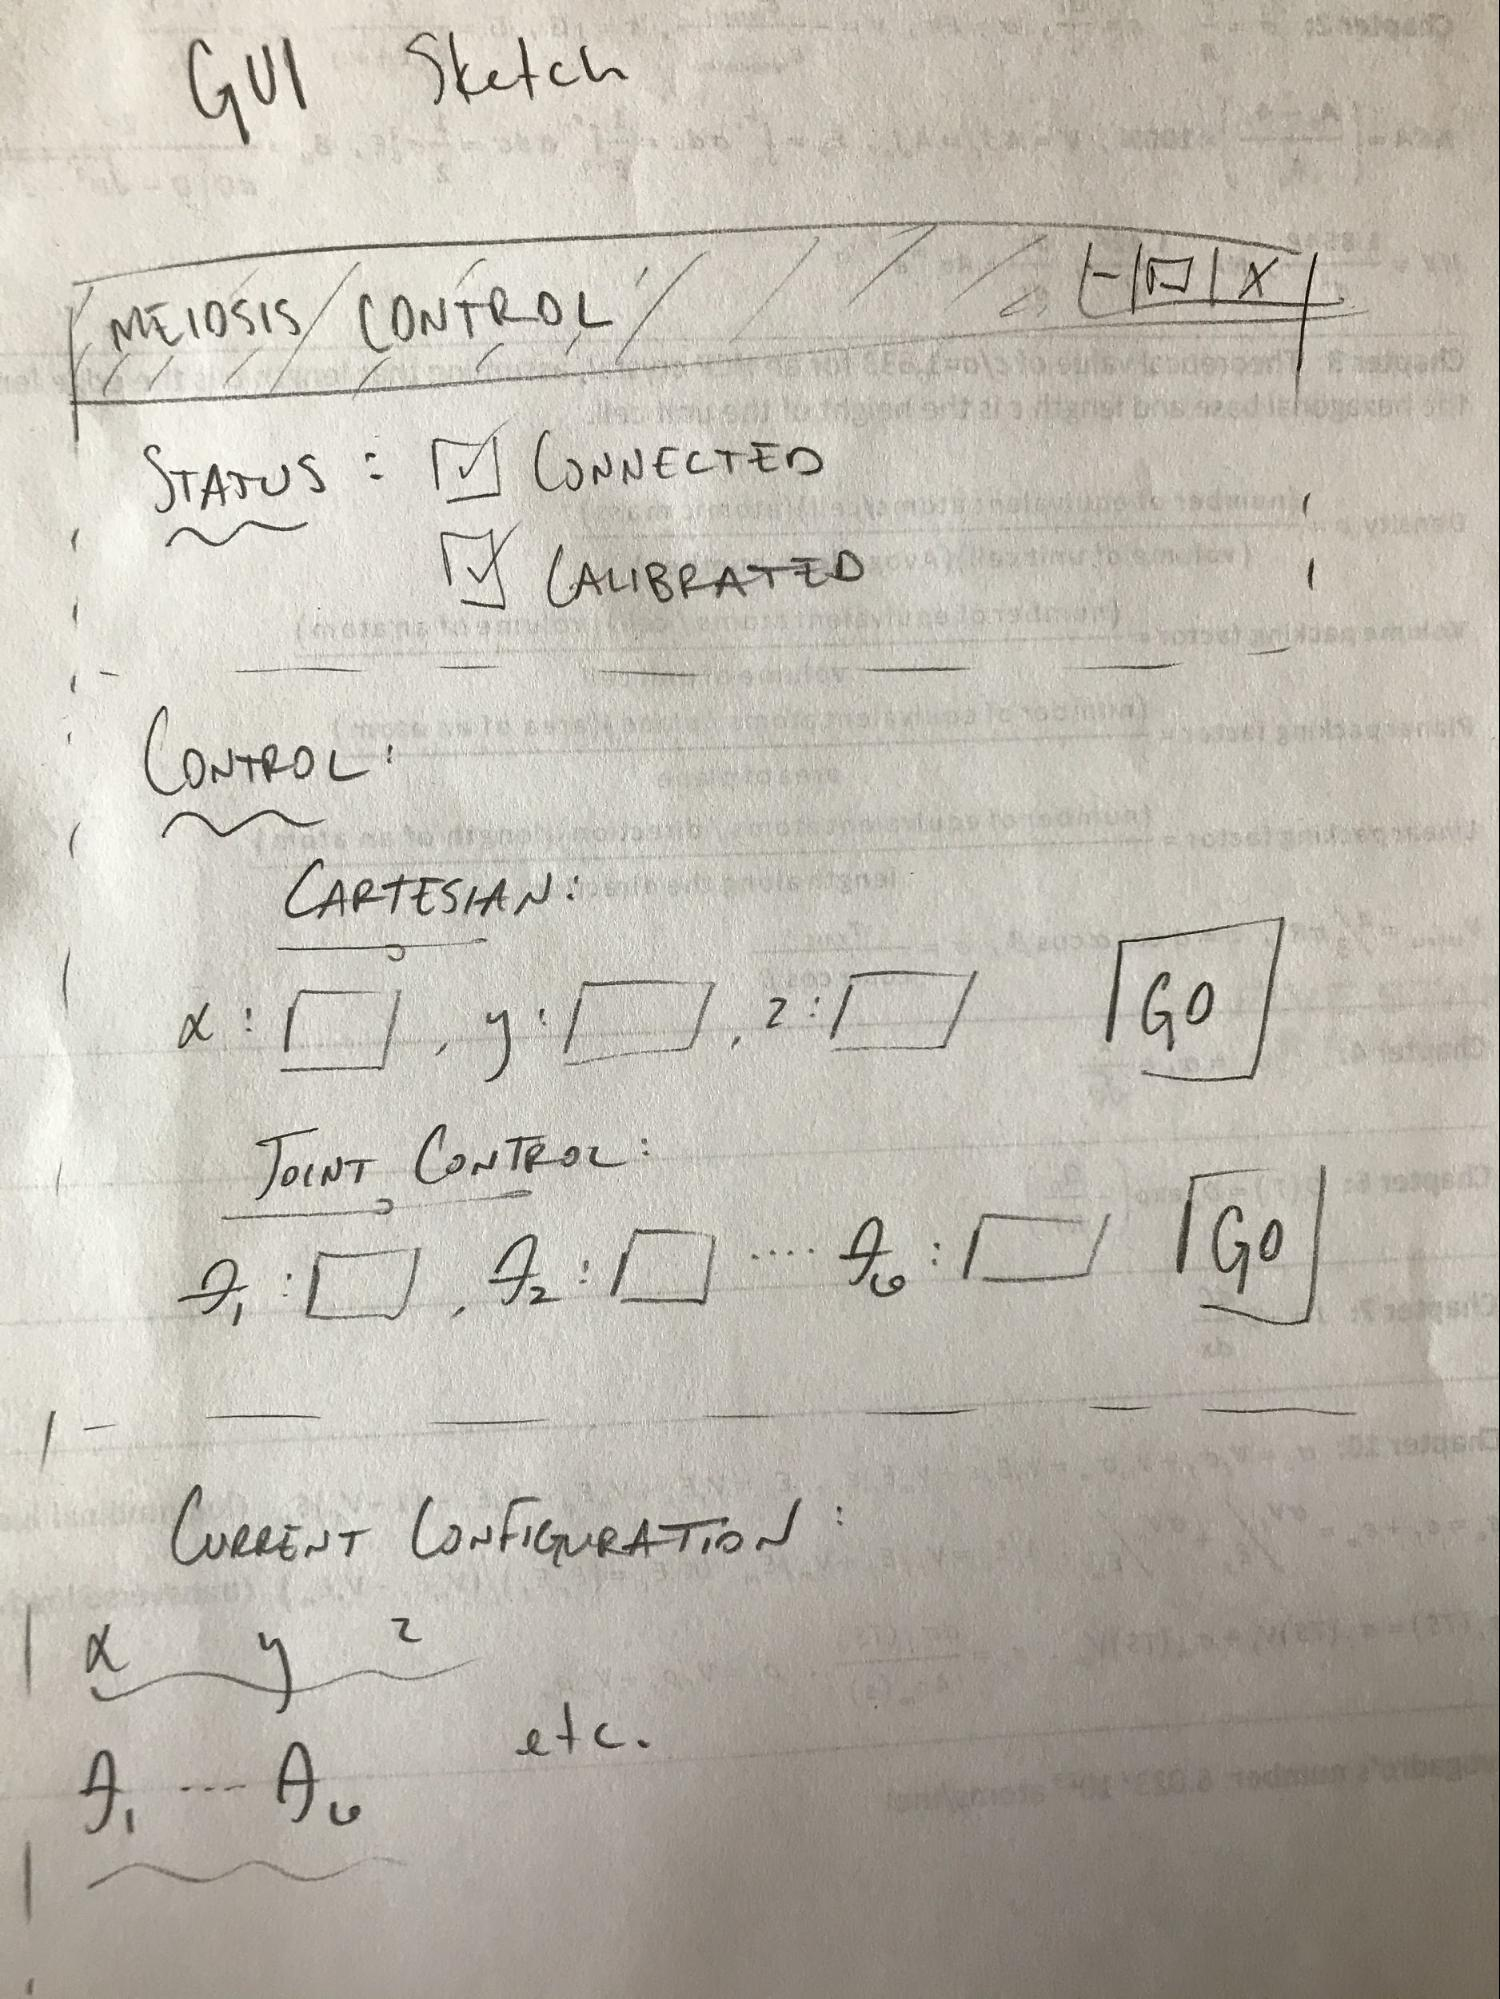
\includegraphics[width=0.5\textwidth,frame]{gui}
  \caption{GUI Template}
  \label{fig:gui}
\end{figure}

As shown in Figure \ref{fig:gui}, the GUI will have desired cartesian end effector positions, such as an X, Y, and Z for the end effector position, as well as an end effector orientation input, i.e., phi, theta, and psi. The input will closely resemble the input of a six element row vector. The interface will also have user selectable direct joint controls, rather than the system performing the inverse kinematic calculations for the user. The interface will also display status indicators showing whether the robot is calibrated as well as the current manipulator configuration.

In order to test this specification, several points within the workspace will be selected as well as at least three points outside of the workspace for the purpose of error checking. The points (in cartesian XYZ and Euler angles) are chosen randomly. These points are then given to the user interface, which will return joint angle values. The same randomly generated coordinates will be given to the verified kinematics functions, and the outputs will be compared to the output of the UI to check for validity.

\newpage
Due to uncertainties in the design caused by recent events, development for this user interface has been stopped and verification of its accuracy can not be determined. Therefore, \textbf{adherence to specification 2.2.a cannot be determined.}


Specification \textbf{2.2.b} states: \textbf{The system shall be capable of performing floating point arithmetic.} In order to fulfill specification 2.2.b, a computational system must be selected that can perform floating point arithmetic. The Raspberry Pi 3b+ includes an ARM Cortex A-53 \cite{rpi}, which is capable of performing high-speed floating point arithmetic \cite{arm}. Based on this fact, \textbf{the manipulator meets specification 2.2b.}


\section{Further Testing}

In order to determine how useful the harmonic gearboxes are, each gearbox must be fatigue tested. The procedures for both the 1/39 ratio gearbox and the 1/20 gearbox are essentially the same, with the only difference being the load applied to each one. To run the test, each gearbox will be fitted with a load that represents the maximum resting force that the individual gearbox will have to support. For the 1/39 gearbox, the weight applied will be equivalent to the weight the manipulator must support in the shoulder joint. For the 1/20 gearbox, the gearbox will be loaded with the weight the manipulator must support in the elbow joint.

Once the load has been applied, the gearboxes will be set to run repeatedly at full speed from 0° to 180°, then back to 0° to maximize the torque being applied to each gearbox. The test will run for eight hours or until the gearbox breaks, after which data will be collected and analyzed.

In order to collect useful data from the fatigue tests, certain measurements must be taken. Before the fatigue test both the height and width of 4 teeth at 90° angles from each other will be measured and marked, then measured again after the tests to determine the wear the gearbox may go through. A visual inspection of the gearbox will also be conducted to determine if there are any shavings of material in the gearbox.

To test how gearbox fatigue will affect error, the PhaseSpace motion capture system will be utilized to determine any drift from the exact angle. Since the length of each load is known, a PhaseSpace marker can be placed at the end of each load so the motion capture system can see the location of the end of the link. The marker will be placed in a slightly recessed divot on the end of the link in order to make the forward kinematics calculations more exact. Another marker will be placed at the center of the motor cap, again placed within a small divot. These markers will allow us to determine the angle of the load by comparing the positions of the end of the load to the center of rotation. While the fatigue test is running, the motion capture system will capture data at each 0 and 180° position, and the actual angle will be plotted versus time to show any drift or error that occurs.

% \newpage
\section{Conclusion}\label{sec:conc}
Table \ref{tab:results} summarizes the results of the tests performed throughout the course of this semester. This table marks whether or not each specification was met or if it could not be determined.

\begin{table}[htp]
  \centering
  \caption{Summary of Test Results}
  \label{tab:results}
  \begin{tabular}{c|c}
  Specification Tested & Specification Met? \\ \hline
  1.1.a & \cmark \\
  1.2.a & \cmark \\
  1.2.b & \cmark \\
  1.3.a & Cannot be Determined \\
  1.4.a & Cannot be Determined \\
  1.4.b & Cannot be Determined \\
  1.4.c & Cannot be Determined \\
  1.5.a & \cmark \\
  1.5.b & \cmark \\
  1.6.a & \cmark \\
  1.6.b & \xmark \\
  1.7.a & \cmark \\
  1.7.b & \cmark \\
  1.8.a & Cannot be Determined \\
  2.1.a & \cmark \\
  2.2.a & Cannot be Determined\\
  2.2.b & \cmark \\
  \end{tabular}
\end{table}

Based on the results of our testing it is not possible to fully determine that the manipulator functions in accordance with the requirements defined. Since specification 1.1.a was met, requirement 1.1, which defines the budget of the robot, is adhered to by the final version of this manipulator. Requirement 1.2 specifies that the manipulator should be fully dexterous without being kinematically redundant. The manipulator is seen in Table \ref{tab:results} to function according to this requirement since both specifications 1.2.a and 1.2.b were tested and met.

Requirements 1.3 and 1.4 both define the necessary precision and accuracy required for this manipulator to be of educational value. The main goal of our project was a robot that is accurate and precise. Since the tests that would determine whether or not the manipulator adheres to these requirements can only be hypothesized and not actually performed, specifications 1.3.a-1.4.c could not be determined and therefore it is unknown as to whether or not the manipulator functions according to requirements 1.3 and 1.4.

The manipulator functions according to requirement 1.5 since specifications 1.5.a and 1.5.b were both met. This requirement details the reachable workspace that the robot should possess. Requirement 1.6 mentions the dexterous workspace that the robot should have available. This requirement was made to ensure that there is enough movement available for the robot to perform tasks. The manipulator was unable to function according to this requirement. The robot is able to adhere to specification 1.6.a, but without a major redesign it does not meet specification 1.6.b.

The robot was tested to meet specifications 1.7.a and 1.7.b and therefore functions according to requirement 1.7, which specifies that the system’s end effector shall be removable and capable of picking and placing a low-odor chisel tip Expo dry erase marker. Since specification 1.8.a could not be determined due to lack of access to the lab it is unsure as to whether the manipulator functions according to requirement 1.8, which mentions that the manipulator should be able to write using the aforementioned Expo marker.

Requirement 2.1, which states that the system shall be open source, has been met since all code and files have been uploaded to a publicly accessible GitHub repository in adherence to specification 2.1.a. However, adherence to requirement 2.2 cannot be determined. Due to the shift out of the lab, there was a large uncertainty as to how the robot would be controlled since there is no longer a physical robot to be moved. This resulted in inconclusive data regarding specification 2.2.a. Despite adhering to specification 2.2.b,  it is unknown as to whether or not the manipulator functions according to requirement 2.2.

Overall, since the success of the manipulator largely depended on the accuracy and precision requirements (1.3 and 1.4), it is not possible to say whether or not the manipulator meets the requirements defined in the preliminary design semester.


\bibliographystyle{plainnat}
\null\newpage\bibliographystyle{ieeetran}\bibliography{robo}\null\newpage
% \bibliography{robo}
\appendix
\renewcommand\thesection{\Roman{section}}
\renewcommand\thesubsection{\roman{subsection}}
\section*{Appendix}\label{sec:app}
% Checks inverse kinematics to verify MEIOSIS robot has the correct
%   dextrous workspace.

clear all
close all
clc

%define resolutions and constants
xres = 5;                  %Cartesion resolution in x direction
tres = 15;                   %Rotational resolution
eOff = [0;0;5.25];          %End effector offset in cm
rInner = 19;                %Inner radius of dexterous workspace
rOuter = 47;                %Outer radius of dexterous workspace
theta = linspace(0,90,91);  %Elevation angle
L = rInner:xres:rOuter;     %Line of points to check
errorPos = zeros(3,length(L),length(theta));
desPos = zeros(3,length(L),length(theta));

for jj = 1:length(theta)
    %Define desired cartesion end effector positions
    desX = cosd(theta(jj)).*L;
    desY = zeros(1,length(desX));
    desZ = sind(theta(jj)).*L + 22.08;

    %Iterate through all positions and orientations
    count = 1;
    for ii = 1:length(desX)
        for tx = deg2rad(0:tres:180)
            for tz = deg2rad(0:tres:360)
                desR = rotz(tz)*rotx(tx);
                desPos(:,ii,jj) = [desX(ii);desY(ii);desZ(ii)];
                [gamma{count},error] = MeiosisIK2(desPos(:,ii,jj),desR);
                if error == 1
                    errorPos(:,ii,jj) = [desX(ii);desY(ii);desZ(ii)];
                    break
                else
                    count = count + 1;
                end
            end
            if error == 1
                break
            end
        end
        if error == 1
            count = count + 1;
        end
    end
    if error == 0
        gammaM(:,:,jj) = cell2mat(gamma);
        for ii = 1:6
            jointMin(ii) = rad2deg(min(gammaM(ii,:,jj)));
            jointMax(ii) = rad2deg(max(gammaM(ii,:,jj)));
        end
        limits(:,:,jj) = [jointMin;jointMax];
    end
end

%Determine the maximum and minimum joint angle requirements
for ii = 1:6
    totalJointLimits(1,ii) = min(limits(1,ii,:));
    totalJointLimits(2,ii) = max(limits(2,ii,:));
end
totalJointLimits

%Error plot
figure(1)
axis equal
axis([-3 52 20 75])
hold on
title('MEIOSIS Dexterous Workspace')
xlabel('x [cm]')
ylabel('z [cm]')

for jj = 1:length(theta)
    for ii = 1:length(L)
        plot(desPos(1,ii,jj),desPos(3,ii,jj),'b.');
        plot(errorPos(1,ii,jj),errorPos(3,ii,jj),'r.');

    end
end

pd = plot(0,0,'b.');
pe = plot(0,1,'r.');
pd.DisplayName = 'Dexterous';
pe.DisplayName = 'Not Dexterous';
legend([pd;pe],'Location','northeast')

print('DexterityWithOffset.pdf','-dpdf')
%
% % Uncomment to animate
% for ii = 1:length(gamma)
%     meiosis_draw(gamma{ii})
%     hold on
%     plot3(desX,desY,desZ,'r.')
%     pause(0.01)
% end



\end{document}
